El pedal de efectos tiene una estructura definida de la siguiente manera: la señal captada atravesará una etapa a la entrada que se encarga de amplificarla y adecuarla para introducirla en la FPGA, donde se procesará. Por último, el resultado será reconvertido en analógico y amplificado para permitir su reproducción.

\section{Captación de sonido: selección de micrófono}

Como normalmente se utilizan pedales de efectos en instrumentos electrófonos, la señal de salida del instrumento ya viaja por un cable de camino a la amplificador, el pedal actúa por tanto como un intermediario entre ambos. Sin embargo, en instrumentos de viento, es necesario utilizar un transductor que sea capaz de convertir la señal acústica consistente en ondas de presión en una serie de impulsos eléctricos que puedan ser procesados posteriormente.

La solución más sencilla consistiría en utilizar el micrófono que viene integrado con la placa Nexys A7: modelo \emph{ADMP421} de Analog Devices~\cite{Nexys}. No obstante, la utilización de este micrófono plantea los siguientes dos problemas.

En primer lugar, es inmediato pensar que incluso en el caso de un prototipo, si se plantea usar como pedal, no resulta nada recomendable colocar el micrófono encargado de recoger todo el sonido en el suelo. Además de estar lejos de la fuente sonora, capturaría el sonido resultante de la manipulación de los controles suponiendo una bajada en la calidad que proporcionase el dispositivo. Por tanto, es mejor utilizar un micrófono no integrado en la propia placa.

\begin{figure}
\begin{center}
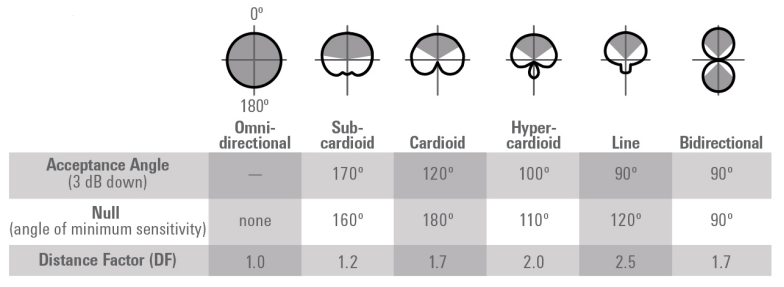
\includegraphics[width=15cm]{img/micros.png}
\caption{\label{fig:polar_dig}Tipos de micrófonos según su diagrama polar~\cite{Mic}}
\end{center}
\end{figure}

En segundo lugar, pero no menos importante, conviene tener en cuenta que la respuesta de sensibilidad del micrófono integrado es omnidireccional (ver figura \ref{fig:polar_dig}), es decir, captará todos los sonidos sin importar la dirección de dónde vengan. Este tipo de transductores se usan principalmente en radio y televisión, donde puede haber varias personas hablando en el mismo micrófono o para la grabación de orquestas o agrupaciones en localizaciones cerradas determinadas. Estos micrófonos son capaces de captar tanto el sonido proveniente de la fuente como los ecos y reflexiones característicos del espacio, dando una sensación de amplitud al oyente como la que produciría su escucha en esa misma localización. Pero mientras que en estos casos se trata de un efecto deseado, resulta poco agradable captar estas reflexiones en un ambiente no preparado para ello y encima cercano al suelo, siendo más conveniente utilizar micrófonos de tipo cardioide.

Estos micrófonos los más utilizados con instrumentos de viento, ya que el sonido suele provenir de un punto concreto. Es preciso matizar que en el caso del saxofón, contra la creencia popular, el sonido no sale siempre por la campana del instrumento. El sonido sale, por el contrario, por la llave abierta más próxima a la embocadura, que suele estar en el centro del cuerpo del instrumento. En consecuencia, no resulta conveniente acercar el micrófono mucho a la campana descuidando otras llaves. La figura \ref{fig:saxo} muestra un saxofón alto aunque hay varios instrumentos de la misma familia.

\begin{figure}[!b]
\begin{center}
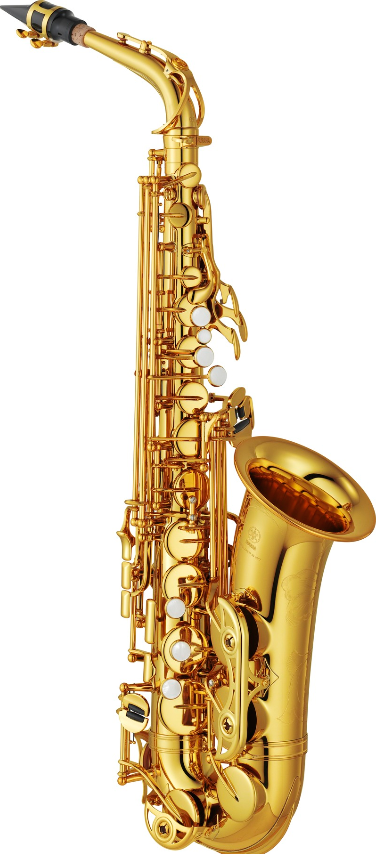
\includegraphics[height=8cm]{img/saxo.png}
\caption{\label{fig:saxo}Saxofón alto}
\end{center}
\end{figure}

Además de tener en cuenta el diagrama polar para la elección de micrófono, resulta imprescindible conocer los posibles tipos en cuanto a fabricación y funcionamiento. En este sentido tenemos los dos tipos más comunes: los micrófonos de condensador y los dinámicos los cuales se describirán brevemente teniendo en cuenta el criterio de \emph{Shure}, uno de los fabricantes de audio profesional más reconocidos del mercado \cite{shuremic}.

Los micrófonos de condensador reciben su nombre del condensador que poseen en el interior de su cápsula. El diafragma es la pieza encargada de vibrar cuando las ondas de presión del sonido lo atraviesan. Esta pieza se une con una de las placas del condensador. El resultado es que con cada movimiento del diafragma varía la distancia entre las placas y en consecuencia, se modifica la capacidad del conjunto de manera inversamente proporcional. Estos cambios modifican una señal eléctrica en la que quedan registradas las ondas de sonido recibidas. Estos micrófonos poseen una buena sensibilidad pero necesitan de alimentación \emph{phantom} de entre 24 y 48 V, que se realiza desde la mesa de mezclas por el mismo cable de señal.

Los micrófonos dinámicos por el contrario, no requieren de alimentación, poseen buena robustez y son más baratos que los anteriores. Estos funcionan gracias a una bobina unida al diafragma que se mueve conforme a las ondas de presión recibidas del sonido dentro de un campo electromagnético. Por la acción de la inducción electromagnética se genera una corriente que atravesará la bobina de manera proporcional al estímulo entrante. La principal desventaja de estos micrófonos es que su respuesta no es del todo lineal con la frecuencia, produciendo mayor o menor ganancia en función del rango del espectro en el que se encuentre el sonido de entrada. Para compensar este efecto se suele usar ecualización posterior o diferentes diafragmas para cada rango del espectro de forma que se pueda reconstruir la señal original a base de sumas de los diferentes tramos.

\begin{figure}[!hb]
\begin{center}
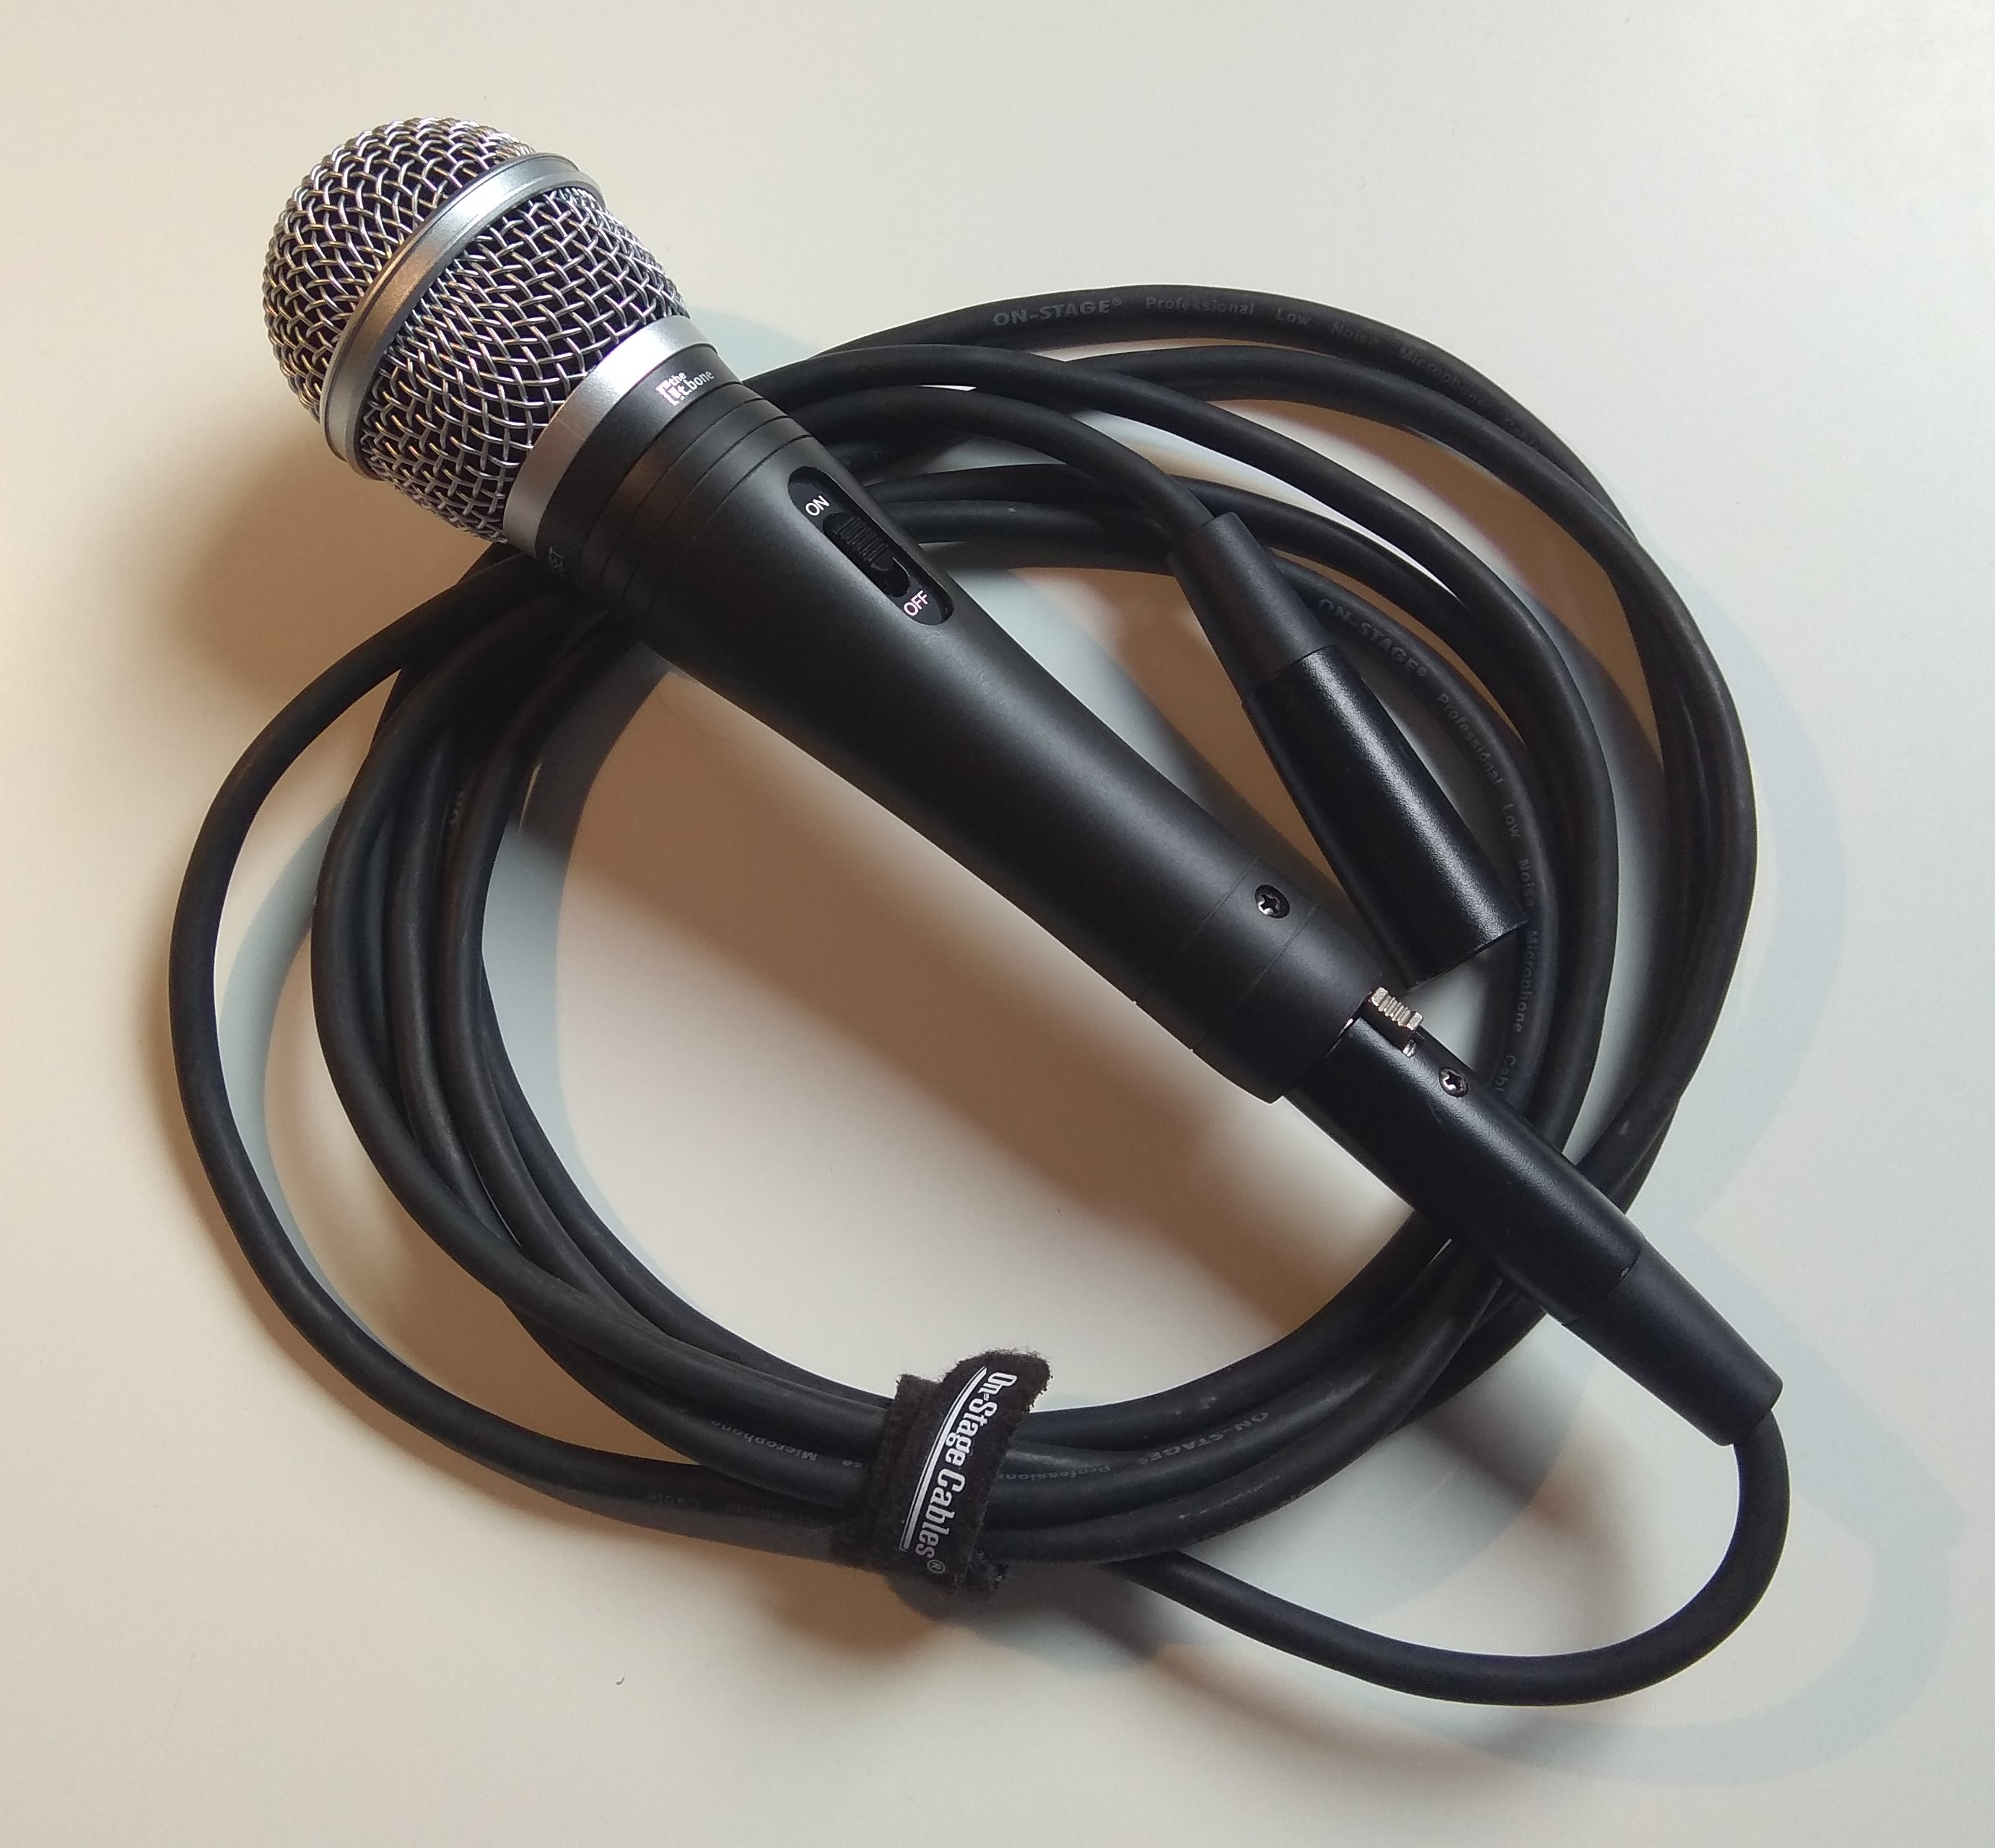
\includegraphics[width=8cm]{img/microusado.jpg}
\caption{\label{fig:microusado}Micrófono utilizado junto con el cable XLR}
\end{center}
\end{figure}

Teniendo en cuenta su uso en el diseño, he escogido un micrófono dinámico por la robustez que presenta que además evitará tener que preocuparse de la alimentación. Adicionalmente, estos micrófonos funcionan de manera muy similar entre sí, lo que resultará muy conveniente para mantener la flexibilidad del proyecto. El micrófono elegido finalmente será un \emph{T.Bone MB60} \cite{tbonemic} cortesía del Club Musical Delta, mostrado en la figura~\ref{fig:microusado}. Este se colocará para capturar los sonidos en un pie en la ubicación más adecuada para el instrumento y se conectará a la etapa siguiente ubicada en el suelo mediante un cable XLR, del que se hablará más adelante.

En cualquier caso, es necesario añadir una etapa posterior de \emph{pre-amplificación o preamp} que adecúe la señal eléctrica del micrófono a otra que pueda interpretar la FPGA. 

\section{Etapa de preamp o preamplificación}

La función principal que va a realizar la etapa de preamplificación será la de transformar la señal balanceada proveniente del micrófono en una sin balancear. Se realizará de manera puramente analógica aprovechando que el esquema está muy desarrollado en la literatura sobre el tema. En este caso he implementado el modelo propuesto por P.Allison en~\cite{Preamp}, el cual fue sugerido por el profesor Alfredo Sanz Hervás al que agradezco su referencia.

Típicamente, los modelos de micrófonos comerciales para aplicaciones de música, utilizan conexiones balanceadas para proporcionar su señal a la salida. El formato de estos cables de 3 hilos recibe el nombre de \emph{XLR} pero también se pueden utilizar conectores de tipo \emph{Jack de 6.35 mm}\footnote{Este tipo de conector pero sin balancear, es el utilizado en guitarras y bajos eléctricos. Para los auriculares se utiliza jack de 3.5 mm que recibe el nombre de ``minijack''.} adecuados a este tipo de señales, ilustrados en la figura \ref{fig:conec}.

\begin{figure}[!htb]
\begin{center}
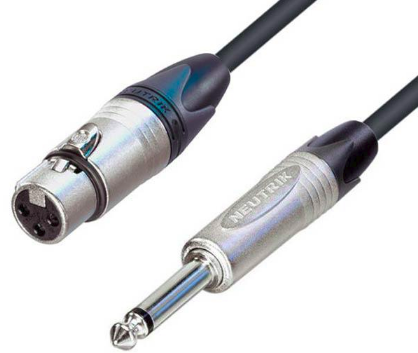
\includegraphics[width=6cm]{img/canonyjack.png}
\caption{\label{fig:conec}Conector tipo XLR hembra y jack no balanceado macho de 6.35 mm}
\end{center}
\end{figure}

El fundamento del par balanceado consiste en enviar la señal por dos conductores entrelazados con la polaridad invertida entre sí, envueltos de un tercer conductor que actúa de barrera frente a interferencias electromagnéticas externas. De esta forma, si se produce una interferencia, afectará a ambos conductores de igual manera. Posteriormente, se introduce la señal en destino en un \emph{Amplificador de diferencias}\footnote{Traducción literal del inglés \emph{Difference Amplifier}, la traducción al castellano puede inducir a error} que se encargará de amplificar únicamente la diferencia entre ambas señales rechazando la interferencia sufrida. Esta idea muy extendida en los diseños analógicos, permite enviar la señal por largos cables de manera robusta a cambio de introducir un tercer conductor. 

Así pues, el diseño de pre-amplificación contará un amplificador de diferencia realizado con un amplificador operacional junto con una pequeña etapa de amplificación mediante transistores BJT, tal y como se puede ver en el esquema del mismo de la figura \ref{fig:circuit}. El potenciómetro permite controlar la ganancia del sistema, es decir, el nivel de señal a la salida del mismo.

\begin{figure}[!thb]
\begin{center}
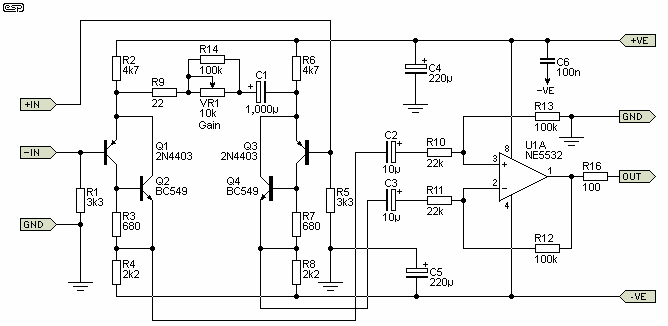
\includegraphics[width=13cm]{img/circuito.png}
\caption{\label{fig:circuit}Esquema del circuito implementado}
\end{center}
\end{figure}

La elección de los transistores y el amplificador operacional pueden condicionar en gran medida el resultado obtenido: es importante que todos los componentes sean robustos frente al ruido. Además, la distorsión que introduzcan puede resultar más o menos agradable al oído. En consecuencia se ha seleccionado un \emph{TL071} \cite{opampdata} por sus características frente al ruido y su reducido precio. Los transistores han sido los mismos que proponía el diseño de P.Allison.

\begin{figure}[!hbt]
\begin{center}
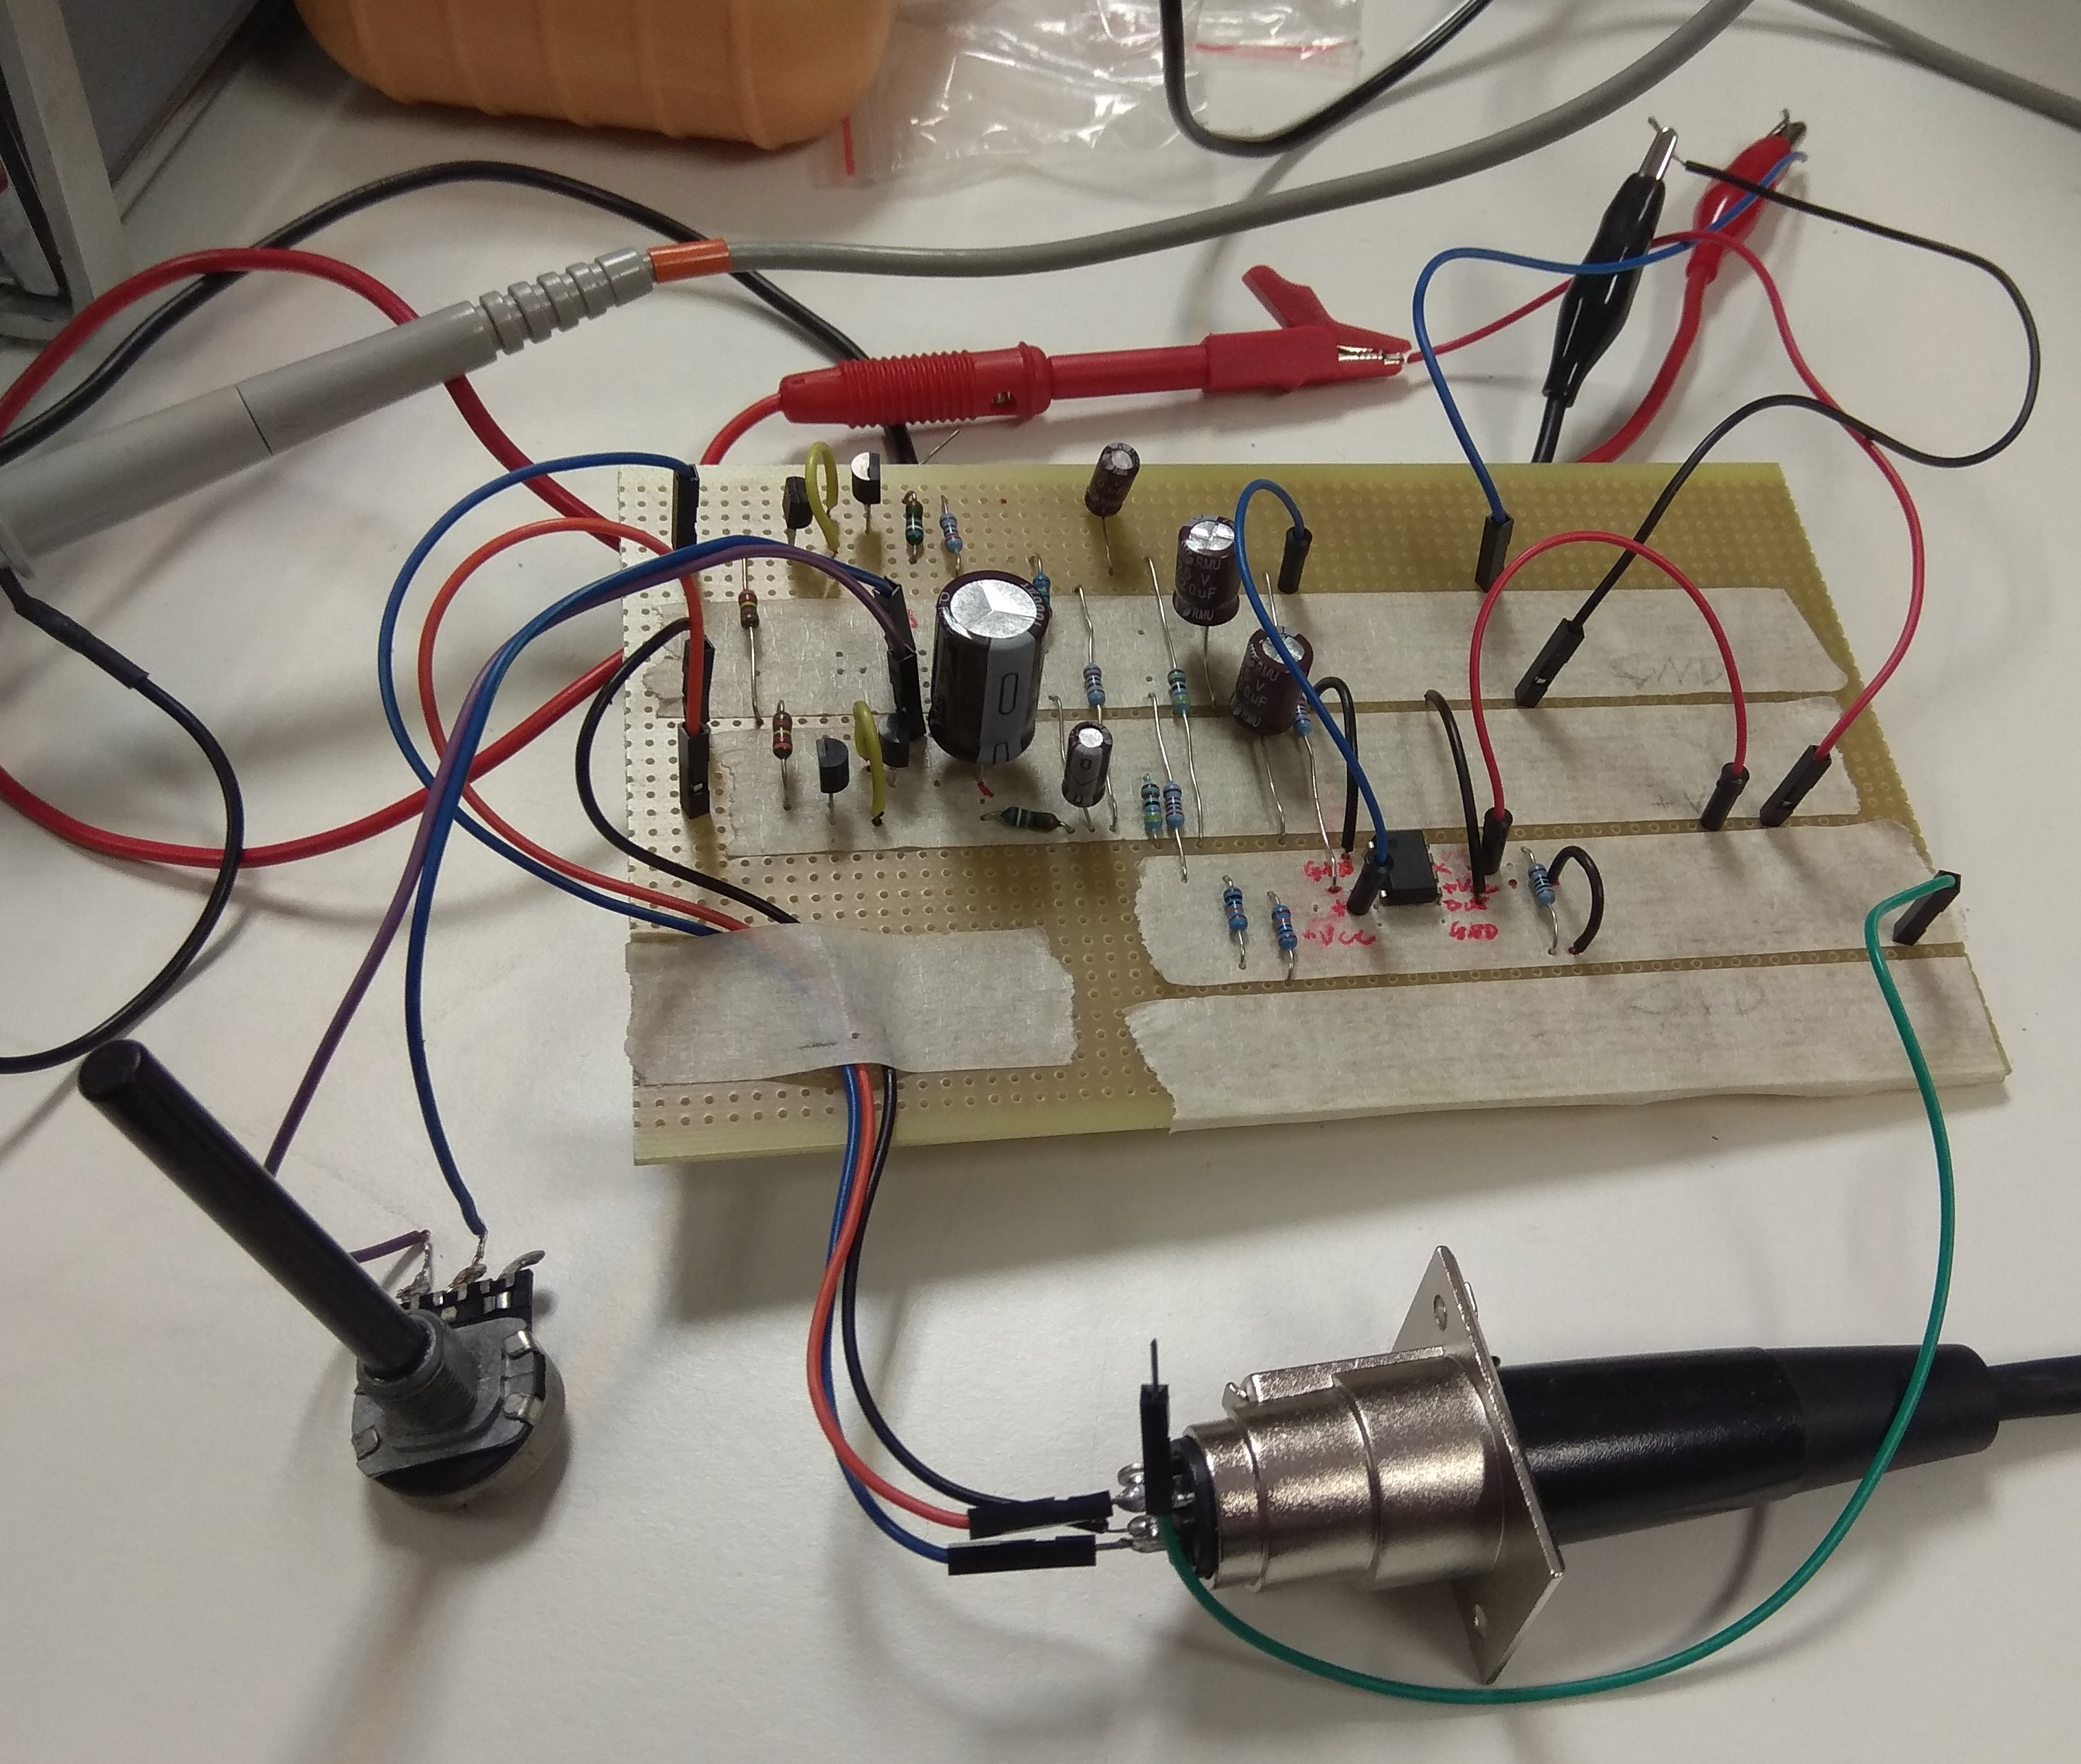
\includegraphics[height=8cm]{img/circuito.jpg}
\caption{\label{fig:placacircuito}Circuito implementado}
\end{center}
\end{figure}

\section{Alimentación}
Para el correcto funcionamiento del circuito es necesario alimentar el operacional y proporcional la polarización adecuada a los transistores. Aunque la bibliografía consultada es ambigua con este tema, finalmente se ha optado por utilizar una alimentación simétrica de $\pm15V$, que será proporcionada directamente de una fuente de alimentación del laboratorio (figura \ref{fig:fuente}). La figura \ref{fig:placacircuito} muestra el circuito una vez montado aunque la caracterización del mismo se describe posteriormente en el punto \ref{testcircuito}.

\begin{figure}[!hbt]
\begin{center}
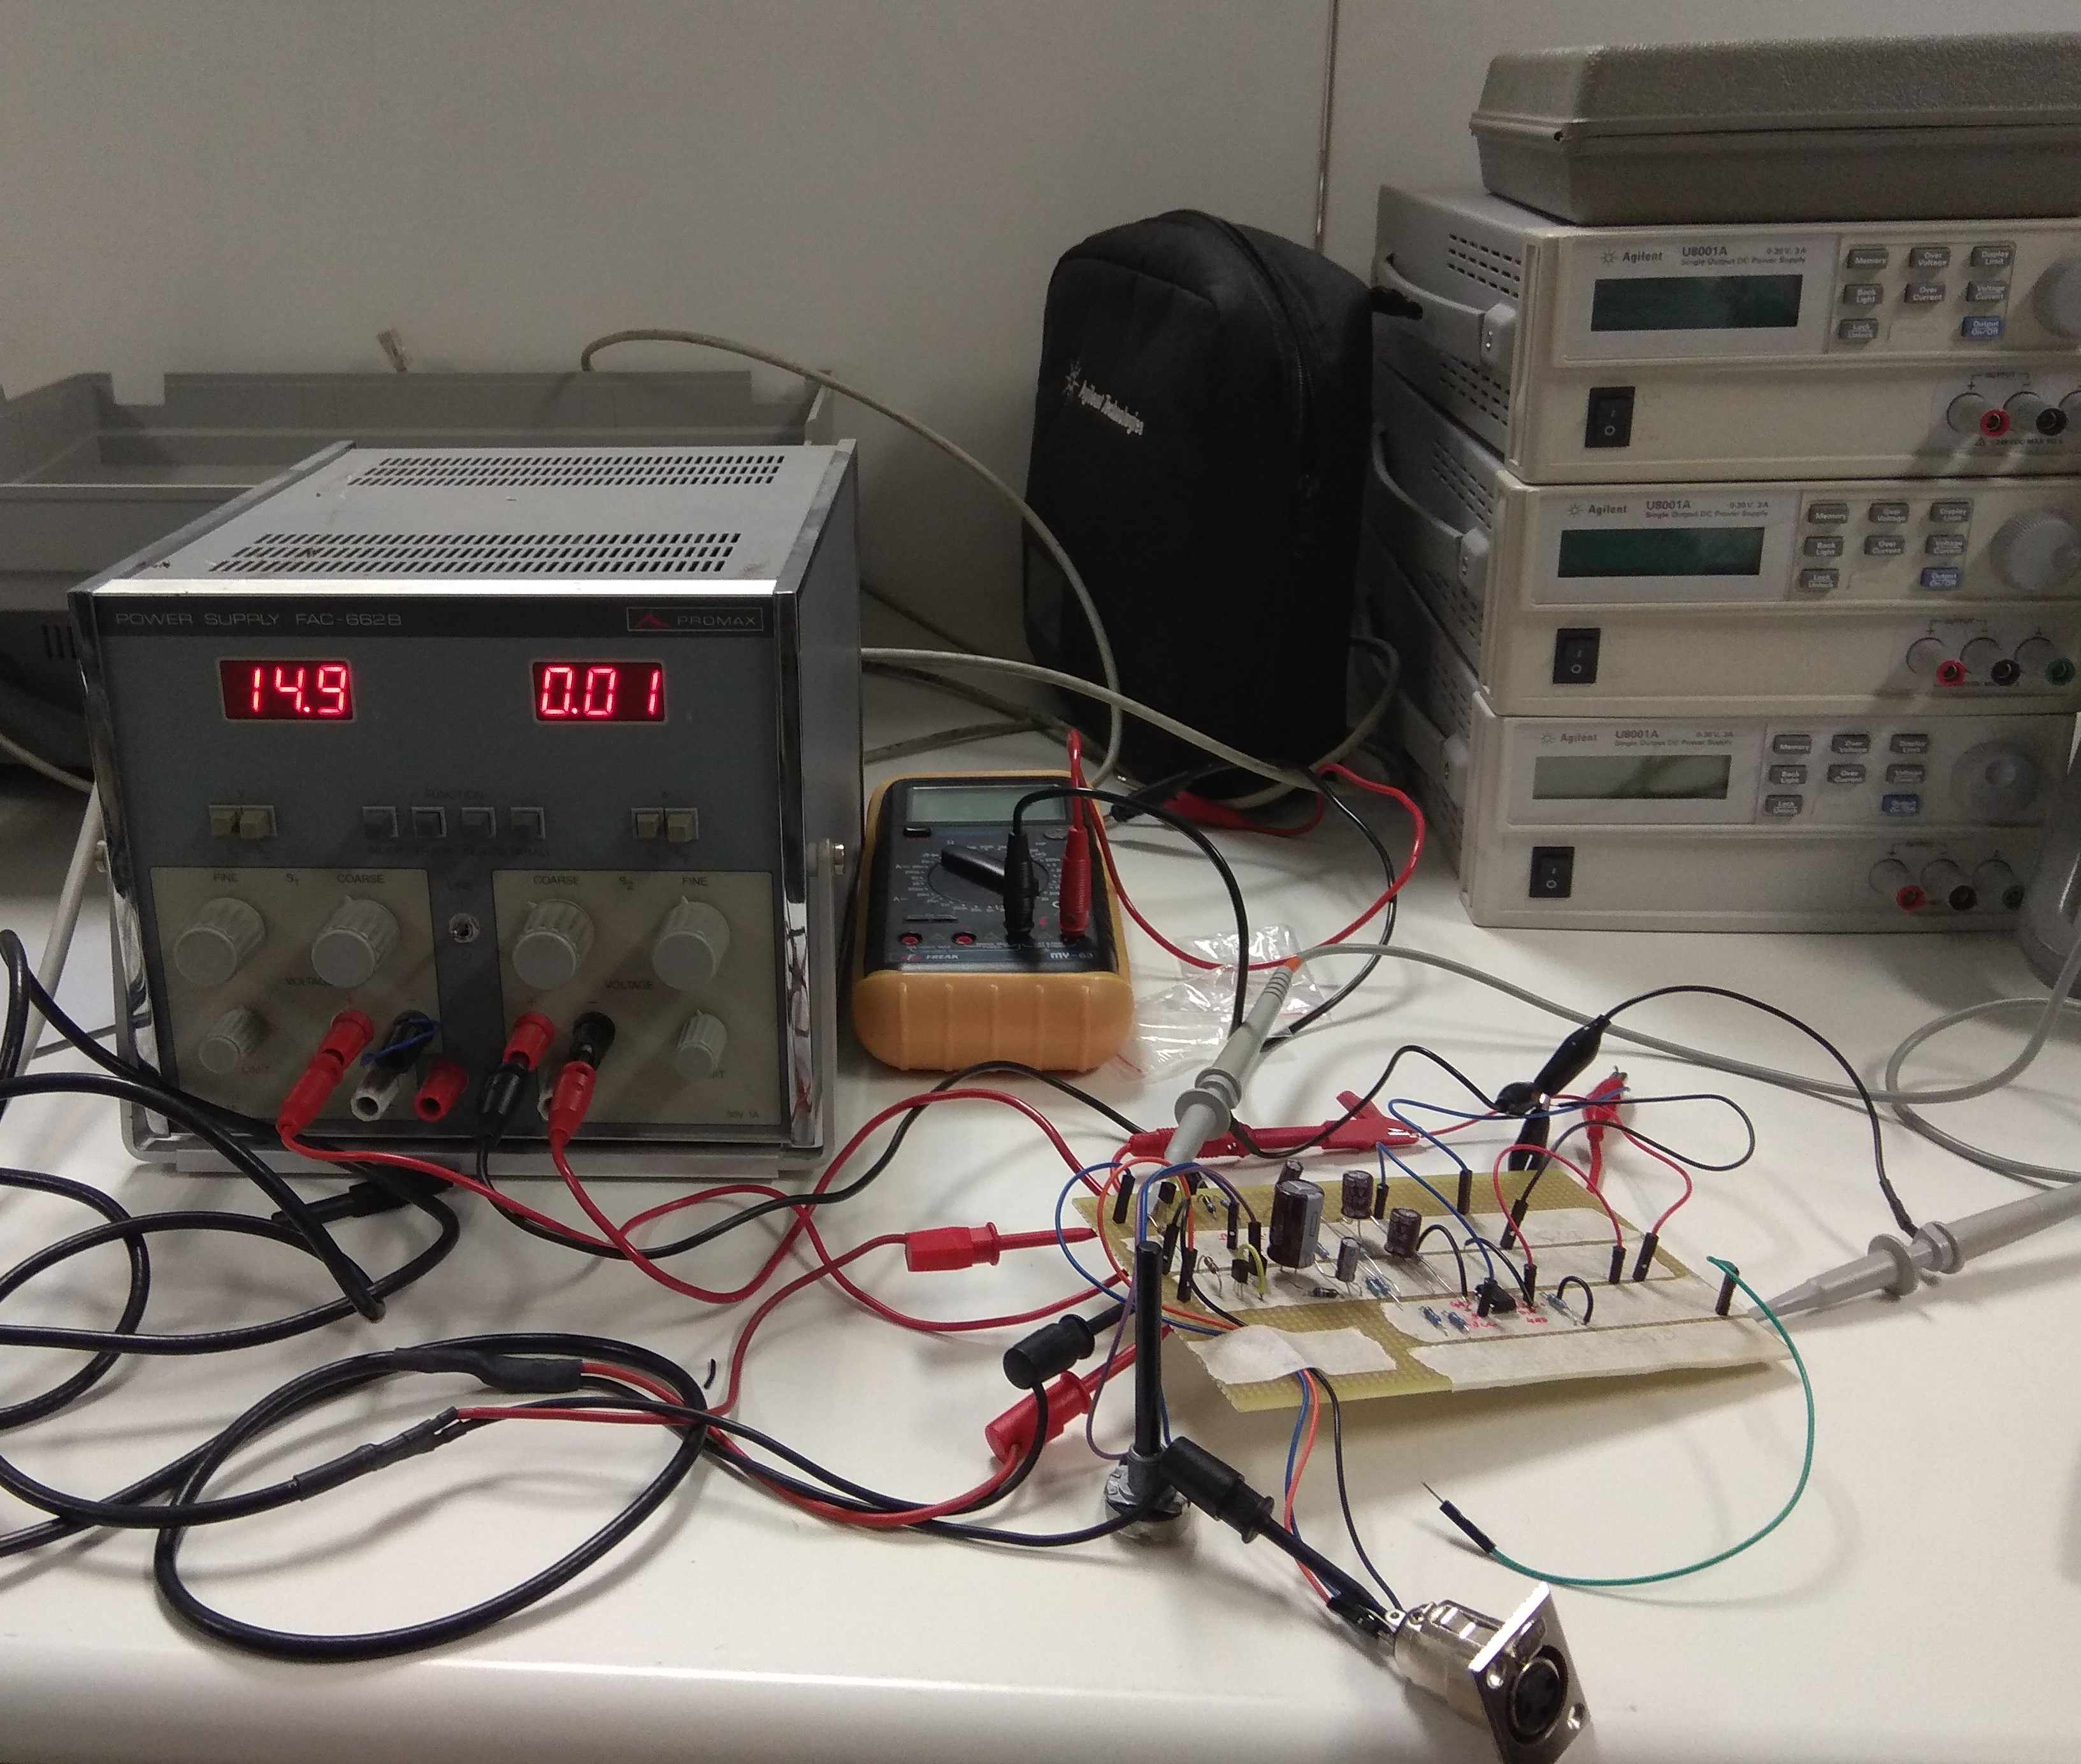
\includegraphics[width=10cm]{img/fuente.jpg}
\caption{\label{fig:fuente}Fuente de alimentación simétrica empleada}
\end{center}
\end{figure}


